\documentclass[10pt,a4paper,onecolumn]{article}
% \usepackage[utf8]{inputenc}
\usepackage{marginnote}
\usepackage{graphicx}
\usepackage{xcolor}
\usepackage{authblk,etoolbox}
\usepackage{titlesec}
\usepackage{calc}
\usepackage{hyperref}
\hypersetup{breaklinks=true,
            bookmarks=true,
            pdfauthor=
{
      Aaron R. Shifman,
  },
            pdftitle=
{
[Re] Ionic Current Model of a Hypoglossal Motoneuron
},
            colorlinks=true,
            citecolor=blue,
            urlcolor=blue,
            linkcolor=blue,
            pdfborder={0 0 0}}
\urlstyle{same}
\usepackage{tcolorbox}
\usepackage{ragged2e}
\usepackage{fontspec}
\usepackage{fontawesome}
\usepackage{caption}
\usepackage{listings}
\lstnewenvironment{code}{\lstset{language=Haskell,basicstyle=\small\ttfamily}}{}



%\usepackage{fancyvrb}
%\VerbatimFootnotes
%\usepackage{graphicx}
%\usepackage{mdframed}
%\newmdenv[backgroundcolor=lightgray]{Shaded}


\usepackage{longtable,booktabs}

\usepackage[
  backend=biber,
%  style=alphabetic,
%  citestyle=numeric
]{biblatex}
\bibliography{shifman-2016.bib}



% --- Macros ------------------------------------------------------------------
\renewcommand*{\bibfont}{\small \sffamily}

\definecolor{red}{HTML}{CF232B}
\newcommand{\ReScience}{Re{\bfseries \textcolor{red}{Science}}}

\newtcolorbox{rebox}
   {colback=blue!5!white, colframe=blue!40!white,
     boxrule=0.5pt, arc=2pt, fonttitle=\sffamily\scshape\bfseries,
     left=6pt, right=20pt, top=6pt, bottom=6pt}

\newtcolorbox{repobox}
   {colback=red, colframe=red!75!black,
     boxrule=0.5pt, arc=2pt, left=6pt, right=6pt, top=3pt, bottom=3pt}

% fix for pandoc 1.14     
\newcommand{\tightlist}{%
  \setlength{\itemsep}{1pt}\setlength{\parskip}{0pt}\setlength{\parsep}{0pt}}

% --- Style -------------------------------------------------------------------
\renewcommand*{\bibfont}{\small \sffamily}
\renewcommand{\captionfont}{\small\sffamily}
\renewcommand{\captionlabelfont}{\bfseries}

\makeatletter
\renewcommand\@biblabel[1]{{\bf #1.}}
\makeatother

% --- Page layout -------------------------------------------------------------
\usepackage[top=3.5cm, bottom=3cm, right=1.5cm, left=1.5cm,
            headheight=2.2cm, reversemp, includemp, marginparwidth=4.5cm]{geometry}

% --- Section/SubSection/SubSubSection ----------------------------------------
\titleformat{\section}
  {\normalfont\sffamily\Large\bfseries}
  {}{0pt}{}
\titleformat{\subsection}
  {\normalfont\sffamily\large\bfseries}
  {}{0pt}{}
\titleformat{\subsubsection}
  {\normalfont\sffamily\bfseries}
  {}{0pt}{}
\titleformat*{\paragraph}
  {\sffamily\normalsize}


% --- Header / Footer ---------------------------------------------------------
\usepackage{fancyhdr}
\pagestyle{fancy}
%\renewcommand{\headrulewidth}{0.50pt}
\renewcommand{\headrulewidth}{0pt}
\fancyhead[L]{\hspace{-1cm}\includegraphics[width=4.0cm]{rescience-logo.pdf}}
\fancyhead[C]{}
\fancyhead[R]{} 
\renewcommand{\footrulewidth}{0.25pt}

\fancyfoot[L]{\hypersetup{urlcolor=red}
              \sffamily \ReScience~$\vert$
              \href{http://rescience.github.io}{rescience.github.io}
              \hypersetup{urlcolor=blue}}
\fancyfoot[C]{\sffamily \thepage}
\fancyfoot[R]{\sffamily Sep 2016 $\vert$
                        Volume \textbf{1} $\vert$
                        Issue \textbf{1}}
\pagestyle{fancy}
\makeatletter
\let\ps@plain\ps@fancy
\fancyheadoffset[L]{4.5cm}
\fancyfootoffset[L]{4.5cm}

% --- Title / Authors ---------------------------------------------------------
% patch \maketitle so that it doesn't center
\patchcmd{\@maketitle}{center}{flushleft}{}{}
\patchcmd{\@maketitle}{center}{flushleft}{}{}
% patch \maketitle so that the font size for the title is normal
\patchcmd{\@maketitle}{\LARGE}{\LARGE\sffamily}{}{}
% patch the patch by authblk so that the author block is flush left
\def\maketitle{{%
  \renewenvironment{tabular}[2][]
    {\begin{flushleft}}
    {\end{flushleft}}
  \AB@maketitle}}
\makeatletter
\renewcommand\AB@affilsepx{ \protect\Affilfont}
%\renewcommand\AB@affilnote[1]{{\bfseries #1}\hspace{2pt}}
\renewcommand\AB@affilnote[1]{{\bfseries #1}\hspace{3pt}}
\makeatother
\renewcommand\Authfont{\sffamily\bfseries}
\renewcommand\Affilfont{\sffamily\small\mdseries}
\setlength{\affilsep}{1em}

\LetLtxMacro{\OldIncludegraphics}{\includegraphics}
\renewcommand{\includegraphics}[2][]{\OldIncludegraphics[width=12cm, #1]{#2}}


% --- Document ----------------------------------------------------------------
\title{[Re] Ionic Current Model of a Hypoglossal Motoneuron}

    \usepackage{authblk}
                        \author[1]{Aaron R. Shifman}
                            \affil[1]{Department of Biology, University of Ottawa, Ottawa, Ontario, Canada}
            
\date{\vspace{-5mm}
      \sffamily \small \href{mailto:ashifman@uottawa.ca}{ashifman@uottawa.ca}}


\setlength\LTleft{0pt}
\setlength\LTright{0pt}


\begin{document}
\maketitle

\marginpar{
  %\hrule
  \sffamily\small
  %\vspace{2mm}
  {\bfseries Editor}\\
  Name Surname\\

  {\bfseries Reviewers}\\
        Name Surname\\
        Name Surname\\
  
  {\bfseries Received}  Sep, 1, 2015\\
  {\bfseries Accepted}  Sep, 1, 2015\\
  {\bfseries Published} Sep, 1, 2015\\

  {\bfseries Licence}   \href{http://creativecommons.org/licenses/by/4.0/}{CC-BY}

  \begin{flushleft}
  {\bfseries Competing Interests:}\\
  The authors have declared that no competing interests exist.
  \end{flushleft}

  \hrule
  \vspace{3mm}

  \hypersetup{urlcolor=white}
  
    \vspace{-1mm}
  \begin{repobox}
    \bfseries\normalsize
      \href{http://github.com/rescience/rescience-submission/article}{\faGithubAlt~Article repository}
  \end{repobox}
      \vspace{-1mm}
  \begin{repobox}
    \bfseries\normalsize
      \href{http://github.com/rescience/rescience-submission/code}{\faGithubAlt~Code repository}
  \end{repobox}
        \hypersetup{urlcolor=blue}
}

\begin{rebox}
\sffamily {\bfseries A reference implementation of}
\small
\begin{flushleft}
\begin{itemize}
    \item[→] \emph{Ionic Current Model of a Hypoglossal Motoneuron}, Purvis LK.,
Butera RJ., (2005) Journal of Neurophysiology, 93, 723--733
  \end{itemize}\par
\end{flushleft}
\end{rebox}


\section{Introduction}\label{introduction}

This work serves as a reference implementation of the model proposed in
\autocite{purvis}, which is a biophysically detailed model of the ionic
currents involved in the rat hypoglossal motoneuron (HM). HMs innervate
the tongue and are involved in breathing, and issues with HMs have been
implicated in sleep apnea\autocite{purvis}. A biophysical model is
derived from known properties, and allows researchers to describe in
detail the role and interactions of all components of the phenomenon.
The model was originally solved (integrated) in XPP and analysed in
MATLAB. This version has been developed in Python both for the fact that
Python is relatively ubiquitous, and the availability of scientific
packages (NumPy, SciPy, \dots). A version of this model exists in cellML
format\autocite{cellml}, however the cellML model is not able to
replicate the original results (action potentials do not occur at 1nA
bias current), nor could it create action potentials with similar
appearance. Due to the nature of the model, debugging is nearly
impossible (multiple variables with the same name i.e. ``theta\_1'').

\section{Methods}\label{methods}

This work was prepared using the authors' description of the model
\autocite{purvis}, and personal communication with the authors. Some
slight inconsistencies were identified in the original paper which had a
negligible effect on the results of the paper. These have been addressed
in this implementation.

The mathematical description of the model was taken directly from page 2
of the original manuscript, and current dynamics were taken from the
appendix. The constants (parameters) were taken from table 2 and the
initial conditions were taken from table 1. It should be noted the the
given initial conditions, while near the equilibrium point (rest), were
not at equilibrium. In order to address this, the model was allowed to
evolve (in the absence of bias current) until numerical equilibrium was
reached, and this was taken to be the initial condition.

While the initial implementation used a Dormad-Prince adaptive solver,
this implementation used the LSODA algorithm (provided in the
scipy.integrate package), with absolute and relative tolerances of
\(10^{-10}\), and a maximum time step of \(\Delta T=0.05\) ms
(convergence of all results was tested with \(\Delta T=0.01\) ms and no
qualitative differences were found). The maximum time step is necessary
in order to account for the relatively short step function current (not
mentioned in the original paper). This implementation used python 3.5.2
(64 bit) on Linux with packages: SciPy v0.17.1, NumPy v1.11.1,
matplotlib v1.5.1.

\section{Results}\label{results}

All results from the original paper have been implemented, however some
slight inconsistencies are noted and will be discussed later.

The first figure in the original paper is the voltage response to a 1
ms, 1 nA current pulse. This is reproduced in figure \ref{fig:fig1}. As
seen, the results are very similar to the original figure, however the
amplitude of the ADP seems a bit below that of the original figure. This
discrepancy will be addressed in the discussion.

\begin{figure}
\centering
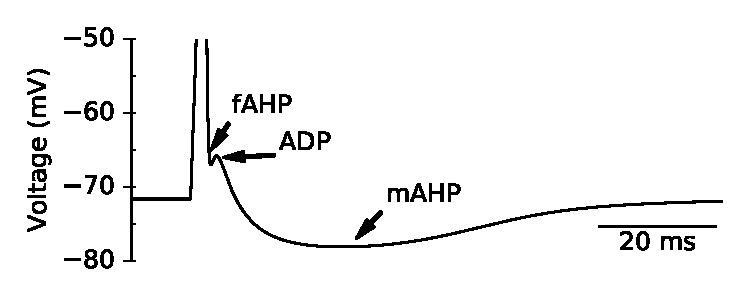
\includegraphics{../code/figures/figure_1.pdf}
\caption{Model response (action potential) to a 1 nA pulse active for 1
ms. Various properties are outlined in the response. \label{fig:fig1}}
\end{figure}

The subsequent analysis performed in the original text is an analysis of
the timescales and amplitudes of the individual ionic currents. This
implementation is recreated in figure \ref{fig:fig2}. This
implementation is very close to the original figure, however it is
important to note that the I-SK current in this implementation has a
peak of \textasciitilde{}0.8 nA, whereas the peak amplitude in the
original paper is \textasciitilde{}1 nA, there are also slight
differences in the calcium currents.

\begin{figure}
\centering
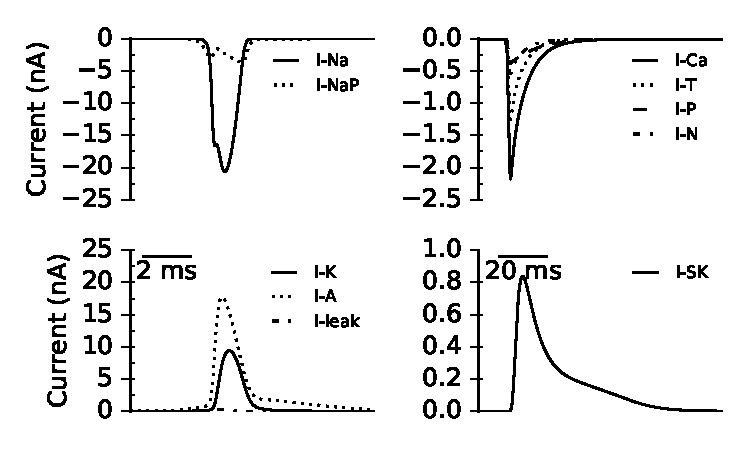
\includegraphics{../code/figures/figure_2.pdf}
\caption{Ionic currents underlying an action potential created by a 1 nA
pulse active for 1 ms. \label{fig:fig2}}
\end{figure}

Figure 3 in the text is an analysis of the dependency of the ADP on
calcium and pre-pulse hyperpolarization. This has been replicated in
figure \ref{fig:fig3}. Again there are slight discrepancies which will
be addressed later.

\begin{figure}
\centering
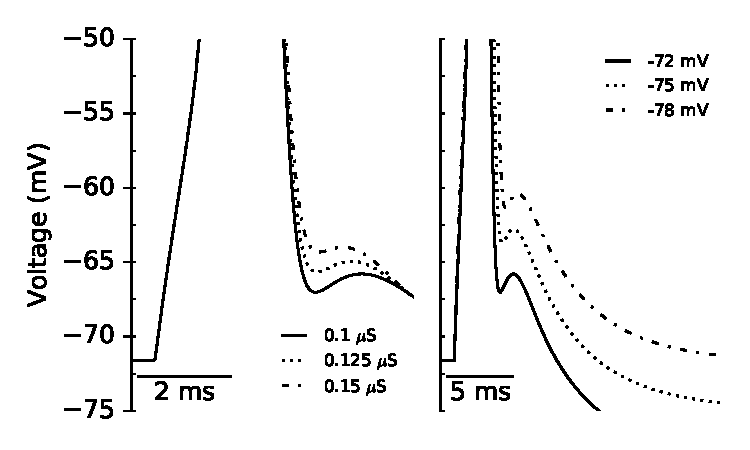
\includegraphics{../code/figures/figure_3.pdf}
\caption{ADP dependancy on calcuim and voltage. Maximal T-type channel
conductance is varied, and resting potential is clamped at a
hyperpolarizing potential. \label{fig:fig3}}
\end{figure}

Validating the model against known experiments, in figure 4 in the text
the authors simulate the application of apamin by eliminating the
SK-current. This result is very well reproduced in figure
\ref{fig:fig4}. The authors also demonstrate spike frequency adaptation
which is known to occur with attenuated SK-current.

\begin{figure}
\centering
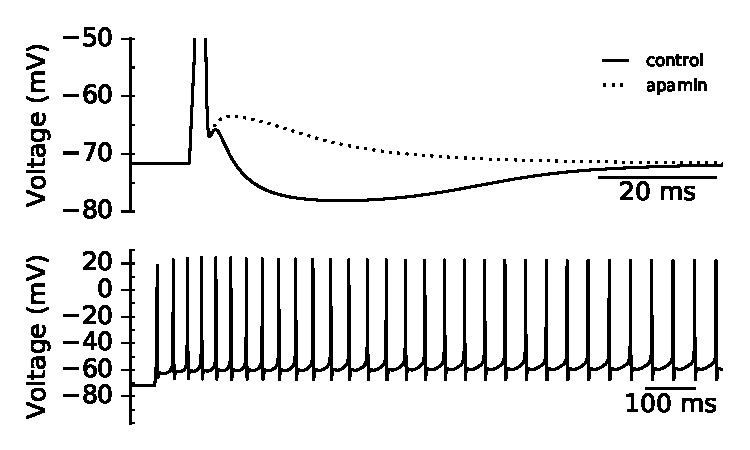
\includegraphics{../code/figures/figure_4.pdf}
\caption{Comparison of model to known experimental results. Removal of
SK-current eliminates the ADP and attenuated SK-currents cause spike
frequency adaptation. \label{fig:fig4}}
\end{figure}

Next, the model response to elongated current application is illustrated
in figure \ref{fig:fig5}, this quite accurately reflects the results
presented in the corresponding plot in the original paper (figure 5).
The action potential plateau is accurately recreated and the length of
the plateau is given by the length of the stimulus (neuron returns to
rest after stimulus is removed). Discrepancies in the length of the
plateau are purely due to discrepancies in the stimulus duration (the
duration used in figure \ref{fig:fig5} is a guess that appears close).

\begin{figure}
\centering
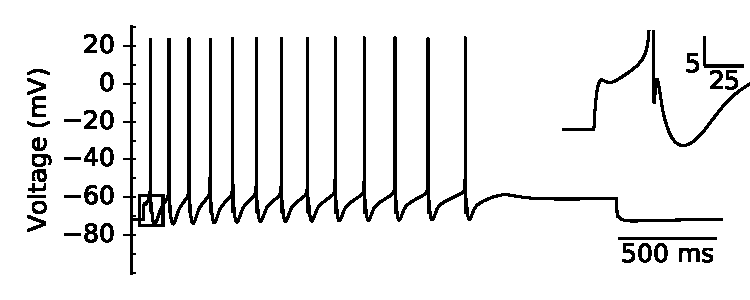
\includegraphics{../code/figures/figure_5.pdf}
\caption{Model response to sustained 0.22 nA pulse which lasts for 2.3
seconds. \label{fig:fig5}}
\end{figure}

The next two figures are an analysis of frequency adaptation of the
neurons under varying T-type calcium currents. In the text figure 7 is
described as having a T-type current 10x that of figure 6. While true,
it would be more accurate to say that figure 6 has a T-type calcium
current 0.1x that of figure 7, as 0.1\(\mu S\) is the ``standard''
conductivity and figure 6 has a conductivity of 0.01\(\mu S\). These
results are quite well replicated in figures \ref{fig:fig6} and
\ref{fig:fig7}. Of note the ``double peak'' as the model stabilizes onto
its sustained spiking behavior is accurately replicated.

\begin{figure}
\centering
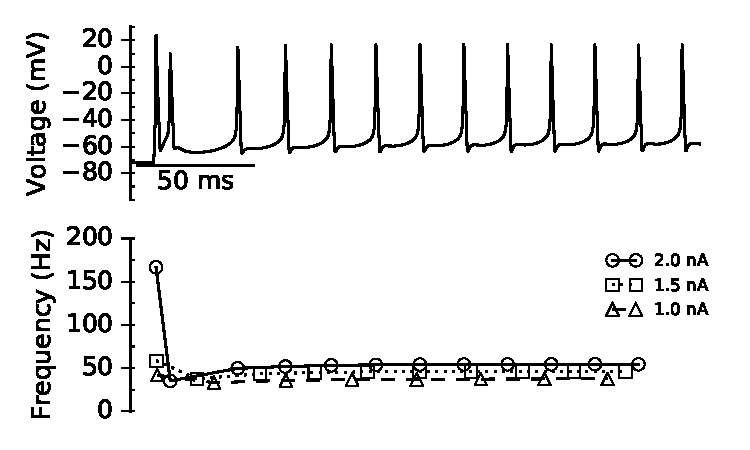
\includegraphics{../code/figures/figure_6.pdf}
\caption{Model response to sustained current step with maximal T-type
conductance of 0.01\(\mu S\) \label{fig:fig6}}
\end{figure}

\begin{figure}
\centering
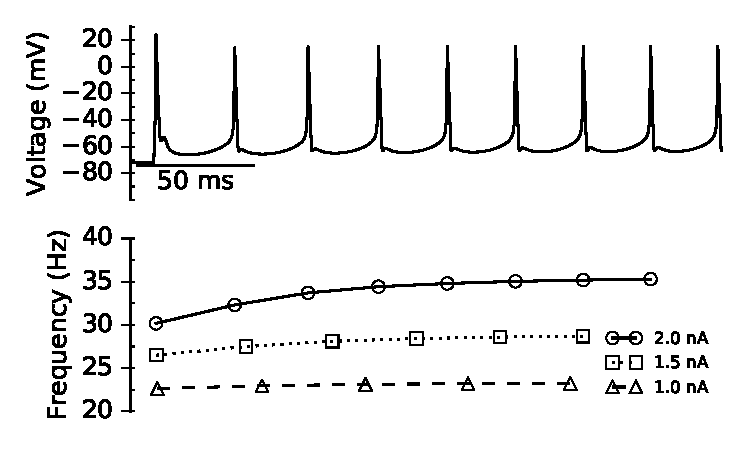
\includegraphics{../code/figures/figure_7.pdf}
\caption{Model response to sustained current step with maximal T-type
conductance of 0.1\(\mu S\) \label{fig:fig7}}
\end{figure}

Following this, spike adaptation is quantified as a function of both
T-type and N-type calcium currents and varying the definition of total
calcium current. These results are very well replicated in figure
\ref{fig:fig8}.

\begin{figure}
\centering
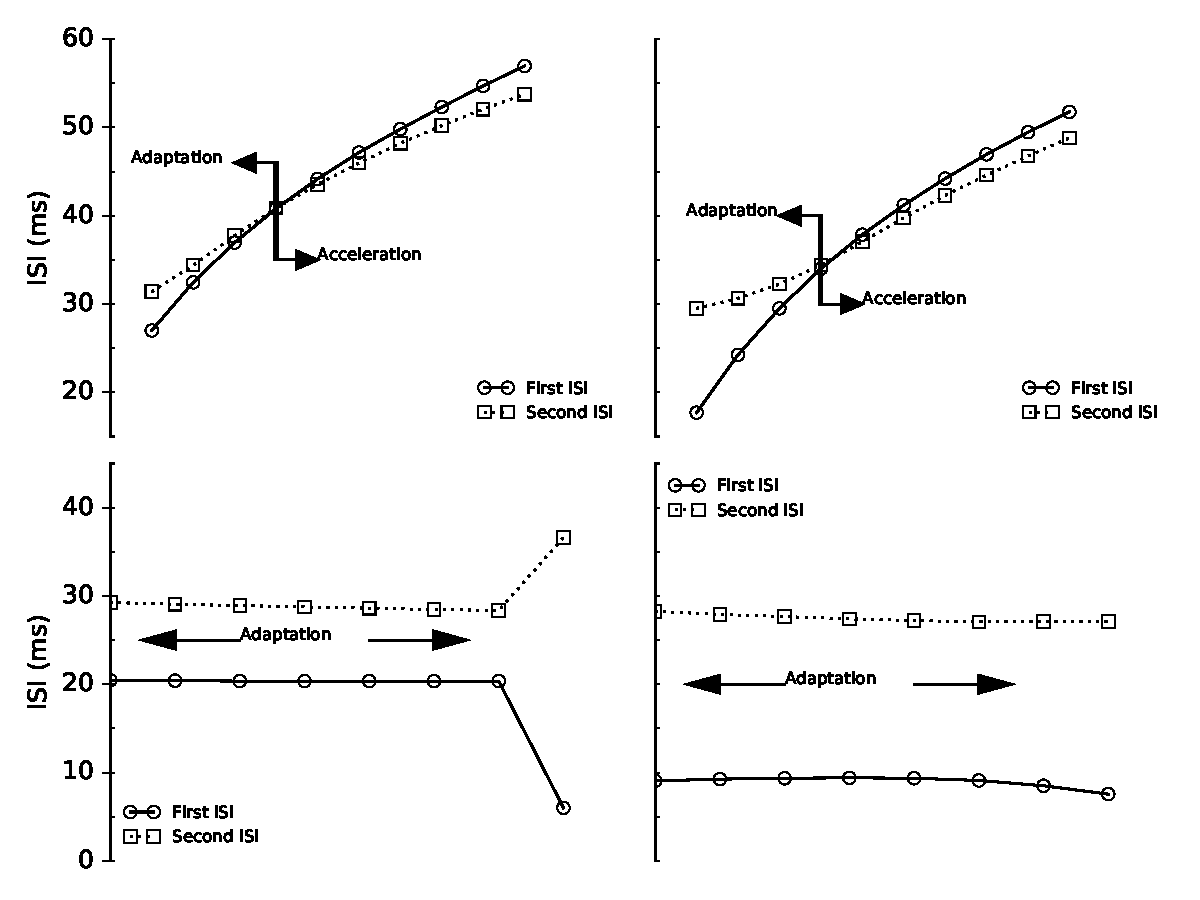
\includegraphics{../code/figures/figure_8.pdf}
\caption{Spike frequency adaptation to various calcium currents
conductances. \label{fig:fig8}}
\end{figure}

The last figure in the text, figure 9, could not implemented solely
based on the description given in the text. In the text the mAHP length
is defined as being ``measured from the repolarizing phase of the action
potential to the point in the AHP that reaches the resting potential''.
Through clarification with the authors, mAHP length is defined as the
length of time between the negative and positive crossing of the resting
potential value.

This is implemented in figure \ref{fig:fig9}, this very closely reflects
the original figure (digitized values provided in the code), however
there are some values that deviate slightly, again this result will be
discussed later.

\begin{figure}
\centering
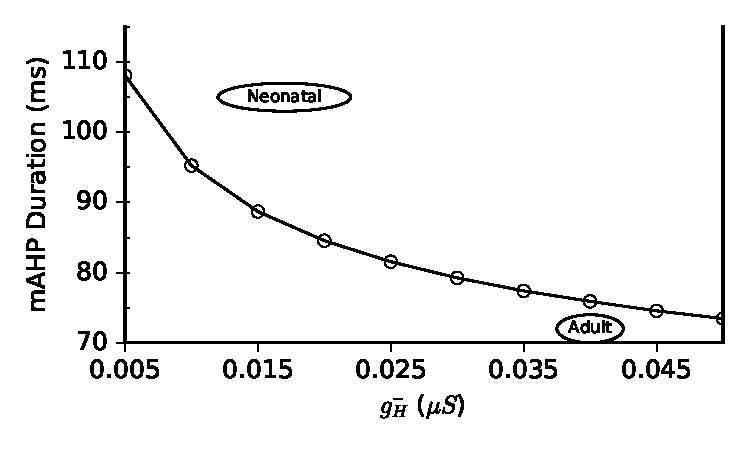
\includegraphics{../code/figures/figure_9.pdf}
\caption{mAHP length as a funtion of H-current amplitude.
\label{fig:fig9}}
\end{figure}

\section{Discussion}\label{discussion}

By and far, this implementation replicates the original paper. Slight
discrepancies in the details however are apparent. For example in figure
\ref{fig:fig1} the ADP amplitude is a few mV different in this
implementation compared to the original. Also for example in figure
\ref{fig:fig2} I-SK is \textasciitilde{}0.8nA in comparison to
\textasciitilde{}1nA in the original. These discrepancies continue
through several other figures. In order to track down these
discrepancies the original authors provided the XPP files they used to
create the figures. The XPP simulation had the same equations and
parameters as this implementation and closely matches this
implementation (code for figure 2 provides the option to compare the
I-SK that XPP calculates with this implementation). Given the fact that
the paper had the same parameters as this implementation and the XPP
simulation matches this implementation, its likely that some simulations
had a slightly different parameter set. For example figures
\ref{fig:fig2} and \ref{fig:fig6} have different parameter sets, and
there are discrepancies in figure \ref{fig:fig2} but not in figure
\ref{fig:fig6}. This may imply that the discrepancies may be in the
differing parameters.

This implementation has identified subtle discrepancies in the original
paper. However this replication proves that all major results:
replication of frequency adaptations, parametric variation, etc\ldots{}
are valid despite these discrepancies.

\section{Conclusion}\label{conclusion}

With confidence, this implementation has indicated that the the original
results were both true, and correctly implemented. This implementation
did identify some subtle discrepancies in the original manuscript, which
were addressed in this implementation.

\section{Acknowledgement}\label{acknowledgement}

I would like to Dr.~Butera for providing the XPP files for the original
paper. Funding for this work was provided in the form of an OGS grant to
ARS from the government of Ontario.

{\sffamily \small
  \printbibliography[title=References]
}
\end{document}
